\documentclass[10pt]{article}

\usepackage[margin=1in]{geometry}
\usepackage{booktabs}
\usepackage{graphicx}
\usepackage{microtype}
\usepackage{xcolor}
\usepackage[colorlinks=true, linkcolor=blue!60!black, urlcolor=blue!60!black, citecolor=blue!60!black]{hyperref}

\newcommand{\plamotok}[1]{\texttt{\textless|plamo:#1|\textgreater}}

\title{Activating Latent Tool-Calling Rails in PLaMo 3:\\
a Data-Centric Case Study on a Laptop}
\author{Gurunath Lunkupali Venugopal}
\date{June 2026}

\begin{document}
\maketitle

\begin{abstract}
We present, to our knowledge, the first open-weights PLaMo model with function calling.
Preferred Networks (PFN) ships tool calling only in its API-only PLaMo Prime line; all
open PLaMo releases are base models. We observe that \texttt{pfnet/plamo-3-nict-2b-base}
(2.6B parameters, attention-only, PLaMo Community License) nevertheless ships an official
\texttt{chat\_template.jinja} and carries undocumented control tokens for chat and
structured output in its vocabulary --- PFN laid the rails but never exposed the capability
in open weights. A small LoRA, trained in 39 minutes on an Apple M4~Pro laptop, activates
those rails: 100\% parse rate, function-name accuracy, and argument exact-match on a
frozen set of 40 unseen call questions, with a 16.7\% false-call rate on 12 strict
no-call cases. The path there is the real story: a contaminated first evaluation
(97.5\% before deduplication, 90\% after), and a v1 training run in which accuracy
\emph{degraded} with more data (90\% $\rightarrow$ 87.5\% $\rightarrow$ 55\%) because 96\%
of the ``no-call'' class was mislabeled by single-turn extraction from a multi-turn dataset.
Fixing the labels --- not adding data or capacity --- produced the final result. We report
honest caveats: with $n=40$, 100\% supports only a $\geq$\,$\sim$91\% lower bound at 95\%
confidence, and the evaluation is in-distribution.
\end{abstract}

\section{Introduction}

PLaMo is Preferred Networks' family of large language models. Tool calling (function
calling) --- the ability to emit a structured JSON invocation of a declared API instead of
prose --- is offered by PFN only through its commercial, API-only \emph{PLaMo Prime} line.
Every open-weights PLaMo release, by contrast, is a base model with no documented chat or
tool capability.

The goal of this study is simple to state: produce the first open-weights PLaMo model with
function calling, on consumer hardware, and document honestly what it took. The result is
a LoRA adapter for \texttt{pfnet/plamo-3-nict-2b-base} that reaches 100\% argument-exact
tool calling on a frozen, leak-free evaluation set of unseen queries --- but the more
useful contribution is the pair of evaluation traps encountered on the way
(Section~\ref{sec:traps}). Both were data problems, not modeling problems, and both would
have silently inflated or destroyed the result had they gone unnoticed. The study is
therefore best read as a data-centric ML case study: the model and the LoRA recipe are
deliberately boring; the data work is where everything happened.

\section{The Hidden Rails}
\label{sec:rails}

The key discovery enabling this work is that \texttt{pfnet/plamo-3-nict-2b-base} (2.6B
parameters, attention-only architecture, PLaMo Community License) is not as ``base'' as
its documentation suggests. Two artifacts ship with the open weights:

\begin{enumerate}
\item \textbf{An official \texttt{chat\_template.jinja}}, defining a role-structured
  conversation format of the form
  \begin{center}
  \texttt{role\plamotok{msg}content\plamotok{tag}}
  \end{center}
  A qualitative probe confirms the base model already follows this template --- it answers
  helpfully in role format --- but it ignores tool-call instructions (e.g.\ asked for the
  weather with a tool schema in context, it explains how to use a weather API rather than
  emitting a call).
\item \textbf{Undocumented control tokens} in the vocabulary, clearly designed for chat
  and structured output (Table~\ref{tab:tokens}).
\end{enumerate}

\begin{table}[ht]
\centering
\caption{Undocumented control-token groups found in the \texttt{plamo-3-nict-2b-base}
vocabulary. None are mentioned in the model card; together with the shipped chat template
they constitute latent infrastructure for chat and structured output.}
\label{tab:tokens}
\small
\begin{tabular}{lll}
\toprule
Group & Tokens & Apparent purpose \\
\midrule
Chat framing      & \plamotok{tag}, \plamotok{msg} & Role/message delimiters (chat template) \\
Structured output & \texttt{key}, \texttt{val} & Key--value emission \\
Constrained decoding & \texttt{choice}, \texttt{constrain} & Choice sets and output constraints \\
Code infilling    & \texttt{fim\_prefix}, \texttt{fim\_suffix}, \texttt{fim\_middle} & Fill-in-the-middle editing \\
\bottomrule
\end{tabular}
\end{table}

The interpretation is that PFN laid the rails for chat, tool use, and constrained
generation in the open checkpoints --- presumably the same scaffolding used to build PLaMo
Prime --- but never trained or exposed the capability in the open weights. The hypothesis
of this study is that a small LoRA can activate those rails cheaply, because the
tokenizer, template, and (plausibly) pre-training distribution are already aligned with
the target format.

\section{Method}
\label{sec:method}

\paragraph{Model and training.}
Base model: \texttt{pfnet/plamo-3-nict-2b-base}. Adapter: LoRA with $r=16$,
$\alpha=32$, applied to all linear layers, with assistant-only loss masking
(loss is computed only on assistant-turn tokens), 1 epoch, bf16, trained on an Apple
M4~Pro via MPS. All runs are tracked in MLflow (SQLite backend,
experiment \texttt{plamo3-tool-calling}) with periodic checkpoints --- the
checkpointing turned out to be essential, as Section~\ref{sec:flaw} shows.

\paragraph{Data.}
Training data is derived from \texttt{glaiveai/glaive-function-calling-v2} (Apache~2.0)
by single-turn extraction: the system message lists the available tool schemas, and the
assistant either answers with a JSON call \texttt{\{"name": ..., "arguments": ...\}} or
gives a plain answer (the ``no-call'' class, included to measure false tool-calls).
Examples are query-level deduplicated. Three training sets appear in this report: the
400-example sprint set (12.5\% no-call), the 11{,}182-example v1 set ($\sim$45\% no-call),
and the 1{,}718-example v2 set (1{,}400 call + 318 strict no-call;
Section~\ref{sec:flaw}). Output format is the official PLaMo~3 chat template throughout.

\paragraph{Evaluation.}
The evaluation set contains 52 cases: 40 questions whose gold answer is a function call
and 12 whose gold answer is to \emph{not} call. Decoding is greedy. Metrics: parse rate
(output parses as a JSON call), function-name accuracy, argument exact-match (no partial
credit), and false-call rate on the no-call cases. The 40 call questions are
\textbf{frozen across all conditions} and have \textbf{zero query overlap with any
training set} (verified). Per-question records --- question, gold, prediction --- are saved
for every condition in \texttt{finetune/results/*.json}, which is what made the failure
analyses in the next section possible.

\section{Two Evaluation Traps}
\label{sec:traps}

We present these not as footnotes but as first-class findings. Both are properties of
the dataset, both were invisible at the aggregate-metric level until inspected, and both
changed the conclusions materially.

\subsection{Trap 1: Eval contamination --- 97.5\% was too good}
\label{sec:contamination}

The first evaluation of the 400-example sprint adapter read \textbf{97.5\%} across parse,
name, and argument metrics. That number was wrong. Investigation showed that
\textbf{41 of the 52 eval queries appeared verbatim in the training data}, because
glaive-function-calling-v2 contains massive row duplication --- naive random splits of
this dataset leak. (After query-level dedup, the entire dataset yields only $\sim$71
unique unseen call queries beyond our training set.) The eval was rebuilt with verified
zero query overlap, and the honest sprint number is \textbf{90\%} argument exact-match.
The contaminated run is archived rather than deleted
(\texttt{results/leaked-eval/}) as a record of the incident.

\subsection{Trap 2: The v1 label flaw --- more data made the model worse}
\label{sec:flaw}

The full v1 run on 11{,}182 examples was expected to improve on the sprint. Instead,
checkpoint evals on the frozen question set showed monotone \emph{degradation} of
argument exact-match: \textbf{90\% (400 ex.) $\rightarrow$ 87.5\% (3.2k ex.)
$\rightarrow$ 55\% (6.4k ex.)} --- see Figure~\ref{fig:flaw}. Two details made this
diagnosable rather than mysterious:

\begin{itemize}
\item \textbf{Precision of emitted calls stayed $\sim$100\%.} At the 6.4k checkpoint,
  every one of the 22 calls the model chose to make was correct (22/22). The model was
  not getting worse at calling --- it was increasingly choosing \emph{not to call}.
  Consistently, the false-call rate also fell (41.7\% $\rightarrow$ 25\% $\rightarrow$
  16.7\%): the model was drifting toward prose on both classes.
\item \textbf{Per-question diffs showed the flips.} Casual zero-argument requests
  (``flip a coin'') flipped from correct JSON calls to polite prose
  (``Sure, let me\ldots'') as training progressed.
\end{itemize}

\textbf{Root cause: 96\% of v1's ``no-call'' class was mislabeled.} glaive conversations
are multi-turn; the assistant frequently first asks a clarifying question or says filler
(``Sure, let me calculate that for you'') and only emits the function call in a
\emph{later} turn. Single-turn extraction labeled all of those first replies ``no-call''
--- systematically teaching the model that tool-worthy requests deserve polite prose.
The run was halted deliberately at step $\sim$870 once the cause was confirmed.

A striking corollary emerged from the audit: under a strict definition of no-call
(no function call \emph{anywhere} in the conversation), \textbf{all $\sim$113k rows of
glaive-function-calling-v2 contain only $\sim$330 genuine no-call conversations}. The
dataset's apparent abundance of negative examples is almost entirely an artifact of
turn slicing.

\begin{figure}[ht]
\centering
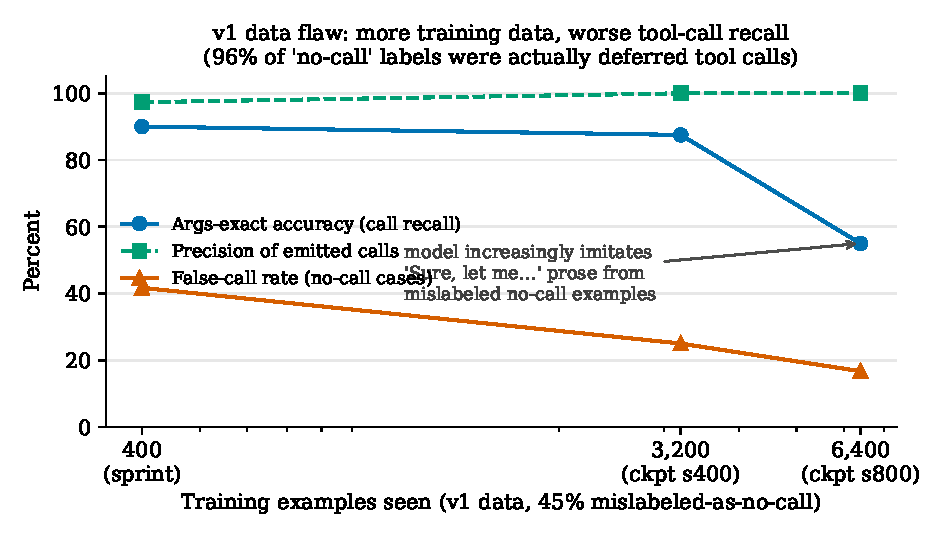
\includegraphics[width=0.78\textwidth]{figures/v1_data_flaw_scaling.pdf}
\caption{The v1 data flaw as a scaling curve: argument exact-match on the frozen
40-question eval \emph{degrades} as the v1 run consumes more mislabeled data
(90\% $\rightarrow$ 87.5\% $\rightarrow$ 55\%), while the precision of the calls the
model still emits stays near 100\%. The run was halted at step $\sim$870.}
\label{fig:flaw}
\end{figure}

\paragraph{The v2 fix.}
v2 rebuilds the no-call class from the $\sim$330 strictly call-free conversations
(318 train / 12 eval) and pairs it with 1{,}400 call examples --- 1{,}718 examples total,
trained in 39 minutes. The deferred-clarification pattern is excluded entirely rather
than mislabeled; modeling it properly is multi-turn behavior (and arguably the
\emph{correct} assistant behavior, which is what PFN's Prime API does) and is left to a
future v3.

\section{Results}
\label{sec:results}

Table~\ref{tab:results} summarizes all conditions on the leak-free evaluation. The 40
call questions are identical in every row.

\begin{table}[ht]
\centering
\caption{Tool-calling results on the frozen, leak-free evaluation (40 call cases +
12 no-call cases; greedy decoding; zero query overlap with training).
$^{a}$\,Trivially low: the zero-shot base model rarely emits a call at all.
$^{b}$\,Measured on 12 \emph{strict} no-call cases (genuinely call-free conversations),
not directly comparable to the v1 rows' column, which inherited the label flaw.}
\label{tab:results}
\begin{tabular}{lrrrr}
\toprule
Condition & Parse & Func-name & Args-exact & False-call \\
\midrule
base, zero-shot                          & 35.0\% & 32.5\% & 0.0\%  & 0.0\%$^{a}$ \\
base, 2-shot                             & 67.5\% & 30.0\% & 0.0\%  & 41.7\% \\
LoRA v1, 400 ex.\ (sprint, 5 min)        & 92.5\% & 92.5\% & 90.0\% & 41.7\% \\
LoRA v1 ckpt @ 3.2k ex.                  & 87.5\% & 87.5\% & 87.5\% & 25.0\% \\
LoRA v1 ckpt @ 6.4k ex.\ (run halted)    & 55.0\% & 55.0\% & 55.0\% & 16.7\% \\
\textbf{LoRA v2, 1{,}718 ex.\ (fixed data, 39 min)} & \textbf{100\%} & \textbf{100\%} & \textbf{100\%} & \textbf{16.7\%}$^{b}$ \\
\bottomrule
\end{tabular}
\end{table}

Three observations:

\begin{itemize}
\item \textbf{Prompting alone cannot do this.} Few-shot prompting raises JSON-shaped
  output (parse rate 35\% $\rightarrow$ 67.5\%) but argument correctness stays at 0\%,
  while the false-call rate jumps to 41.7\%.
\item \textbf{The sprint headline holds after decontamination:} a 5-minute LoRA on 400
  examples takes argument-exact tool calling from 0\% to 90\% on unseen queries.
\item \textbf{Data quality beat data quantity by a wide margin:} v2's 1{,}718 clean
  examples (100\%) outperform v1's 6{,}400 flawed examples (55\%) with under a third of
  the data and 39 minutes of laptop training.
\end{itemize}

\begin{figure}[ht]
\centering
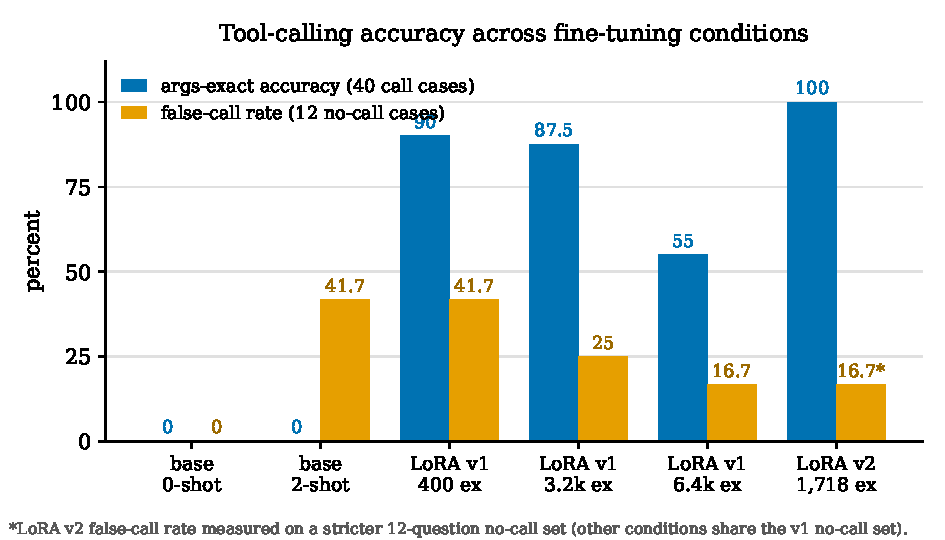
\includegraphics[width=0.85\textwidth]{figures/fig1_conditions.pdf}
\caption{Args-exact accuracy (40 call cases) and false-call rate (12 no-call cases)
across all six conditions. The base model cannot tool-call at any argument-exact level;
the v1 checkpoints trace the label-flaw degradation; v2 reaches 100\% args-exact with
the lowest false-call rate. The v2 false-call bar is measured on the stricter no-call
set (see Table~\ref{tab:results}).}
\label{fig:conditions}
\end{figure}

\begin{figure}[ht]
\centering
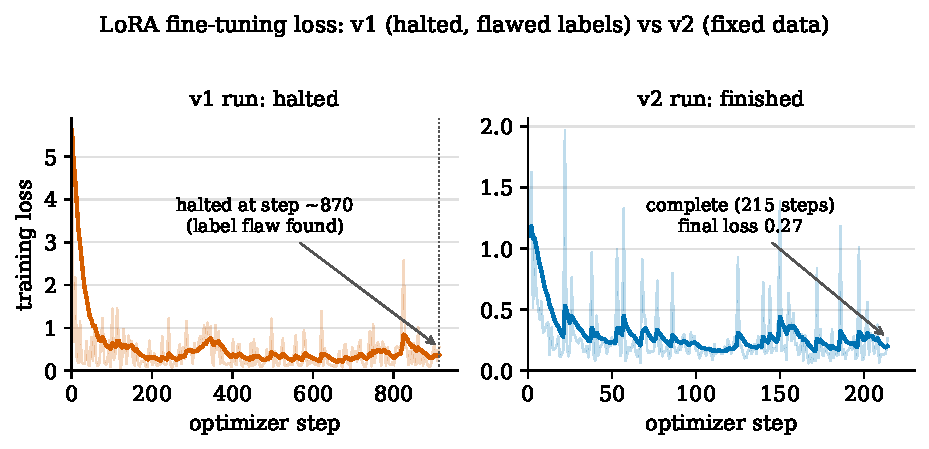
\includegraphics[width=0.95\textwidth]{figures/fig2_losscurves.pdf}
\caption{Training loss versus optimizer step from MLflow. Left: the v1 run, halted at
step $\sim$870 when the label flaw was found --- note that the loss curve itself looks
perfectly healthy, which is exactly why checkpoint \emph{evals} (not loss) caught the
problem. Right: the v2 run on fixed data, completing 215 steps with final loss 0.27.}
\label{fig:loss}
\end{figure}

\begin{figure}[ht]
\centering
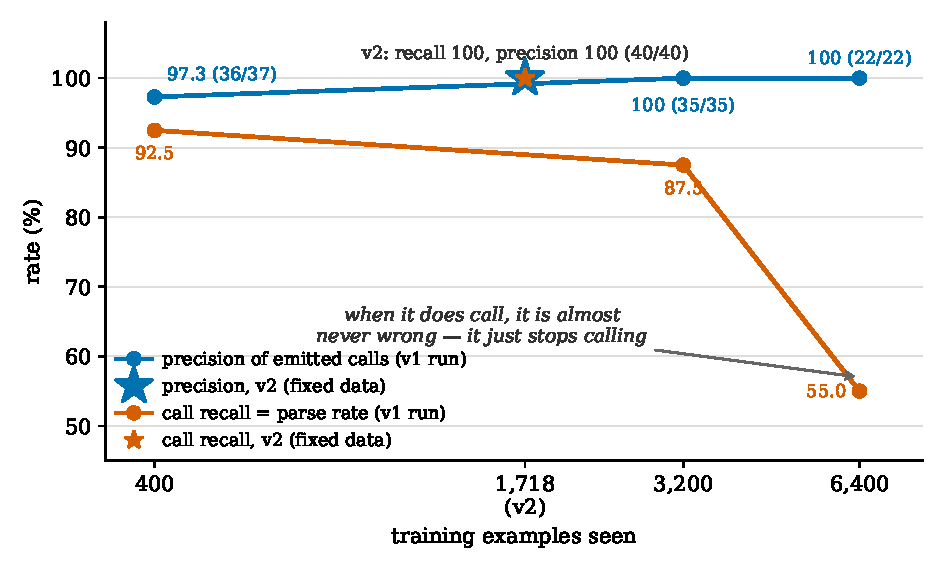
\includegraphics[width=0.85\textwidth]{figures/fig3_precision_recall.pdf}
\caption{Precision--recall decomposition of the v1 failure. As the v1 run sees more
mislabeled data, call recall (= parse rate on call cases) collapses from 92.5\% to 55\%,
but the precision of the calls the model still emits stays at or near 100\%
(36/37 $\rightarrow$ 35/35 $\rightarrow$ 22/22). When it does call, it is almost never
wrong --- it just stops calling. The v2 star recovers both: recall 100, precision 100
(40/40).}
\label{fig:pr}
\end{figure}

\section{Analysis}
\label{sec:analysis}

\paragraph{Precision versus recall, not capability loss.}
The v1 degradation is best understood as a precision--recall trade driven entirely by
label noise (Figure~\ref{fig:pr}). The mislabeled no-call class supplied a strong,
consistent gradient toward prose on tool-worthy inputs; the model obliged by lowering
its propensity to call while its calling \emph{competence} --- conditional on deciding to
call --- remained intact ($\sim$100\% precision throughout, 22/22 at the worst
checkpoint). This is a useful diagnostic pattern in general: when a metric collapses,
decomposing it into ``does the model attempt the behavior'' and ``is the attempt
correct'' distinguishes a decision-boundary shift from genuine capability loss.

\paragraph{The remaining v2 failure mode is hallucinated functions, not over-eagerness.}
v2's 16.7\% false-call rate is 2 misses out of 12 strict no-call cases. Both are
tool-adjacent requests (e.g.\ ``calculate my loan payment'') where \emph{no matching
tool was listed} in the system message --- the model hallucinated a plausible function
name and arguments instead of declining. This is a different and arguably harder failure
mode than the v1-era one (calling when prose is wanted): it is a failure to ground the
call decision in the \emph{provided} schema list. Negative examples that pair
tool-adjacent queries with non-matching schemas are the obvious v3 data intervention.

\section{Limitations}
\label{sec:limitations}

These caveats bound what the 100\% row in Table~\ref{tab:results} can and cannot claim.

\begin{itemize}
\item \textbf{Small $n$.} With 40 call questions and zero errors, the rule of three
  gives a 95\%-confidence lower bound of only about 91\% --- ``100\%'' should be read as
  ``$\geq$\,$\sim$91\% at 95\% confidence'', not as perfection.
\item \textbf{In-distribution evaluation.} Eval queries are synthetic glaive-style
  English, and 39 of the 40 eval functions were seen in training \emph{by name} (new
  queries and new argument values, but the same schemas). The verified zero query
  overlap means the result reflects \emph{distribution-narrowness, not
  example-memorization} --- but it is still in-distribution generalization.
\item \textbf{Novel-tool generalization untested.} A BFCL-style evaluation with held-out
  schemas would be required to claim generalization to unseen tools.
\item \textbf{English-only training data; single seed;} exact-match argument scoring
  with no partial credit; single-turn behavior only (no multi-turn clarification, the
  pattern deliberately excluded in v2).
\end{itemize}

\section{Reproducibility}
\label{sec:repro}

\paragraph{Artifacts.}
\begin{itemize}
\item Adapter weights and per-question eval records:\\
  {\small\url{https://huggingface.co/Gurunath/plamo-3-nict-2b-tool-calling-lora}}\\
  (v2 at the repo root; the 400-example sprint adapter in \texttt{checkpoint-400/}).
\item Code and study log:\\
  {\small\url{https://github.com/rajagurunath/pfn-plamo-inference-study}}
\item MLflow: experiment \texttt{plamo3-tool-calling} (SQLite backend,\\
  \texttt{mlflow ui --backend-store-uri sqlite:///mlflow.db}) contains the sprint run,
  the two killed v1 runs (\texttt{lora-r16-n11182}), and the finished v2 run
  (\texttt{lora-r16-n1716}).
\end{itemize}

\paragraph{Commands.}
\begin{verbatim}
python prep_data.py        # build data/{train,eval}.jsonl from glaive-v2
python train_lora.py       # ~40 min on M4 Pro MPS -> adapter/
python eval_tools.py --condition base
python eval_tools.py --condition base-fewshot
python eval_tools.py --condition lora
\end{verbatim}

\paragraph{Licensing.}
The base model is under the PLaMo Community License; the
\texttt{glaive-function-calling-v2} training data is under Apache~2.0.

\end{document}
